\documentclass[11pt,english]{article}
\usepackage[T1]{fontenc}
\usepackage[latin9]{inputenc}
\usepackage{geometry}
\geometry{verbose,tmargin=1.5cm,bmargin=1.5cm,lmargin=1.5cm,rmargin=1.5cm}
\setlength{\parskip}{\bigskipamount}
\setlength{\parindent}{0pt}
\usepackage{babel}
\usepackage{color}
\usepackage[capposition=top]{floatrow}
\usepackage{placeins}
\usepackage{subcaption}
\usepackage{array}
\usepackage{multirow}
\usepackage{amsmath}
\usepackage{amssymb}
\usepackage{graphicx}
\usepackage{afterpage}
\usepackage{rotating}
%\usepackage{epstopdf}
\usepackage[outdir=./]{epstopdf} % Specify the output directory for pdf figures that are converted from eps. Without this, latex cannot read eps figures on mac.
%\usepackage{epstopdf}

\usepackage{esint}
\usepackage[authoryear]{natbib}
\usepackage[unicode=true,pdfusetitle,
bookmarks=true,bookmarksnumbered=false,bookmarksopen=false,
breaklinks=false,pdfborder={0 0 1},backref=false,colorlinks=false]
{hyperref}
\hypersetup{
	citecolor=red,urlcolor=red,linkcolor=red}
\setcounter{MaxMatrixCols}{10}

\setcounter{MaxMatrixCols}{10}

\geometry{verbose}
\PassOptionsToPackage{normalem}{ulem}
\hypersetup{
	plainpages=false,urlcolor=magenta,citecolor=magenta,linkcolor=blue,pdfstartview=FitH,pdfview=FitH,plainpages=false,urlcolor=blue,citecolor=blue,linkcolor=blue,pdfstartview=FitH,pdfview=FitH}



\makeatletter

%%%%%%%%%%%%%%%%%%%%%%%%%%%%%% LyX specific LaTeX commands.
%% Because html converters don't know tabularnewline
\providecommand{\tabularnewline}{\\}

%%%%%%%%%%%%%%%%%%%%%%%%%%%%%% User specified LaTeX commands.


\newcommand*{\FigDir}{../figures} % Folder where figures are stored

\def\indep{\perp\!\!\!\perp}


\def\limfunc#1{\mbox{\rm #1}\,}
\def\d{\,\mathrm{d}}

\usepackage{fullpage}
\usepackage{amsfonts}
\usepackage[titletoc]{appendix}
\usepackage[font=small,labelfont=bf]{caption}
\usepackage{booktabs}
\makeatother

\begin{document}

\title{Tax Avoidance Paper: Report V47}
\maketitle

\section{No Avoidance Experiments \label{sec:exp}}

\begin{itemize}
	\item Experiment 3: No avoidance on both margins (i.e. no income shifting and all entrepreneurs are taxed as sole-prop.)
	\item Experiment 4: No avoidance on both margins, and the policy function for occupational and legal form choice is fixed at the benchmark model.
	\item (new) Experiment 5: All entrepreneurs are sole proprietors (same financial frictions and same taxes).
	\item (new) Experiment 6: All entrepreneurs face the same borrowing constraint as pass-through businesses. Corporations can engage in income-shifting.
\end{itemize}



\begin{table}[htbp]
	\centering
	\begin{tabular}{lcccc}
		\toprule
		& {Exp. 3} & {Exp. 4} & {Exp. 5} & {Exp. 6} \\ 
		\midrule
		\multicolumn{5}{l}{\textit{\underline{Impact on prices}}} \\
		Interest rate (p.p.) & -0.54 &-0.19 & 0.10 & 0.10  \\
		Wage (\%) & 3.47 & 1.20 & -0.58 & -0.59 \\
		\midrule
		\multicolumn{4}{l}{\textit{\underline{Impact on aggregates}}} \\
		Aggregate output (\%) & 7.26 & 1.80 & -2.91 & -2.88 \\
		
		Aggregate capital (\%)& 10.07 & 4.33 & -2.27 & -2.24 \\
		Ave. entrepreneurial capital (\%) & 39.77 & 9.72 & -13.94 & -13.61 \\
		Entre. share of output (p.p)    & 11.34 &  1.22 & -5.04 & -5.09 \\
		\midrule
		\multicolumn{4}{l}{\textit{\underline{Impact on taxes}}} \\
		Total revenue (excl. soc. sec. \%) & 6.23 & -1.51 & -9.53 & -9.62 \\
		Social security contributions (\%) & 3.47 & 1.20 & -0.58 & -0.59 \\
		Social security tax rate (p.p.) & -0.85& -0.61 & -0.67 & -0.47 \\

		\midrule
		\multicolumn{4}{l}{\textit{\underline{Impact on entrepreneurial sector}}} \\
		Share of entrepreneurs (p.p.) & -0.51 & -0.37 & 0.42 & 0.35 \\
		Sole prop.~as share of entre. (p.p.)    & -35.24 &-0.72 & 32.52 & 12.24  \\
		S-corp.~as share of entre. (p.p.)       & -24.18 & -0.34 & -24.18 & -3.89 \\
		 C-corp.~as share of entre. (p.p.)       & 59.41 & 1.05 & -8.34 & -8.34 \\
		\bottomrule
	\end{tabular}
	\caption{The Impact of Tax Avoidance: Counterfactual Experiments}
	\label{tab:exp_summary}%
	\floatfoot{\textit{Notes:} The table shows the outcomes of the counterfactual experiments relative to the benchmark economy either in \% or in p.p.  Exp.~3 and Exp.~4 refer to a tax reform that taxes all entrepreneurs as sole proprietors. Exp.~4 fixes the occupation and legal form of business organization at the benchmark economy: $o(a, \epsilon, \theta,z_{-})\equiv o^b(a, \epsilon, \theta,z_{-})$. Exp.~5 assumes all entrepreneurs are sole proprietors. All model and tax parameters are at their benchmark values. The social security tax adjusts such that social security contributions equal total pension expenses. To highlight the effects of eliminating tax avoidance on tax revenue, we do not adjust the income tax parameter $\lambda_i$ to balance the government budget constraint. Assuming fiscal neutrality does not change the qualitative results except for total tax revenue. }
\end{table}


\begin{figure}[htbp]
	\centering

		\centering
		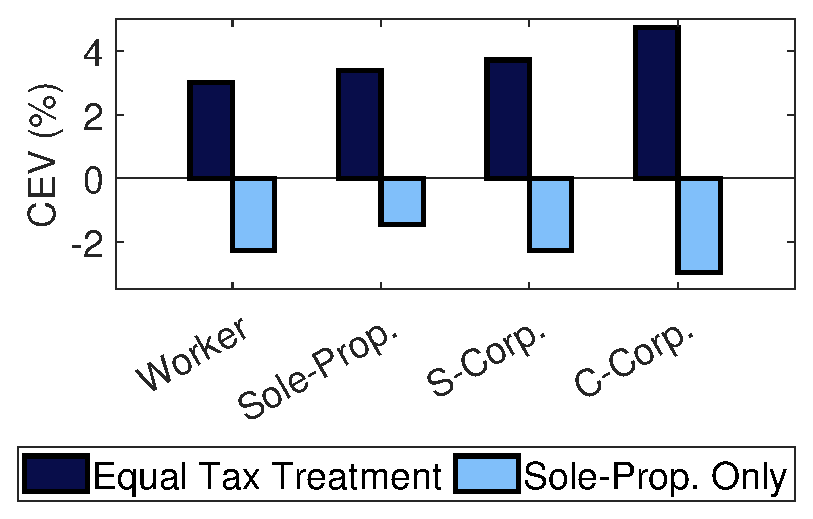
\includegraphics[width=0.6\textwidth]{\FigDir/exp/cev_z_exp_taxreform}
		\caption{CEV by occupation and LFO}
	\label{fig:exp_cev}
	\floatfoot{\textit{Notes:} We assume fiscal neutrality in counterfactual economies and consider transitional dynamics. Each wealth bin contains a quarter of the young population, ordered from the poorest to the richest.}
\end{figure}



%\bibliographystyle{aer}
%\bibliography{DKST_biblio2}
	
\end{document}
